\documentclass[a4paper]{article}
\usepackage{geometry}
\usepackage{graphicx}
\usepackage{amsmath,amssymb}
\usepackage{times}
\usepackage[hidelinks]{hyperref}
\usepackage{fancyhdr}
\usepackage{pgfplots}
\pgfplotsset{compat=1.18}
\urlstyle{rm}
\setlength\parindent{0pt}
\geometry{top=1in,inner=1in,outer=1in,bottom=1in,headheight=3em,headsep=2em,footskip=3em}
\pagestyle{fancyplain}
\lhead{\fancyplain{}{Assignment 4}}
\rhead{\fancyplain{}{ECE 759 HPC}}
\cfoot{\thepage}
\title{\textsc{Assignment 4}}
\author{Sammarth Kapse \\ 9088922829 \\
\url{https://github.com/sammarth-kapse/repo759/tree/main/HW04}}
\date{}
\begin{document}
\maketitle

\section*{Task 1}
I ran the supplied \texttt{nbody.py} locally without changing its source. It uses
$N=100$, $t_{\mathrm{end}}=10$, $\Delta t=0.01$, and seed 17. The saved final
particle/trail plot is submitted separately as \texttt{task1.png}.

\section*{Task 2}
The serial C++ program completes the supplied skeleton. For each particle it computes
\[
 \mathbf a_i=G\sum_{j\ne i}m_j
 \frac{\mathbf r_j-\mathbf r_i}
 {(\|\mathbf r_j-\mathbf r_i\|^2+\epsilon^2)^{3/2}}.
\]
The constants are $G=1$, $\epsilon=0.1$, $\Delta t=0.01$, and board limits $[-4,4]$.
Velocities are converted to the center-of-mass frame. Each timestep applies a half kick,
drifts and clamps positions, recomputes acceleration, and applies the second half kick.
The timestep count follows the supplied C++ skeleton.

\section*{Task 3}
OpenMP parallel loops distribute particles among threads. Every force-loop iteration
owns one output acceleration and keeps its summation over other particles serial.
The implicit barriers finish each stage before the next stage uses its results.
\texttt{schedule(runtime)} and \texttt{OMP\_SCHEDULE} select static, dynamic, or guided
without changing the required command-line interface. Both C++ versions use seed 17;
NumPy and C++ generators produce different initial samples, so their plots need not coincide.

\textbf{Validation:} On Euler, 60 force checks, 50 full-trajectory checks, and 10 invalid-input checks passed. The largest position difference from an independent Python reference was $4.44\times 10^{-16}$. Both required compile commands worked without loading additional modules. Per-step CSV output is disabled in benchmark builds.
\newpage
\section*{Task 4}
All experiments used Euler node \texttt{euler01.engr.wisc.edu}, Slurm job 108475, and exactly eight requested CPUs. The workload was $N=256$, $t_{\mathrm{end}}=100$, $\Delta t=0.01$ (10000 timesteps). Each point is the median of 3 fresh-process runs. Timings include C++ initialization, the initial acceleration, and the simulation loop; CSV I/O and printing are excluded.

\begin{center}\begin{tabular}{lrrrr}\hline
Policy & 1 thread (ms) & 8 threads (ms) & Best $t$ & Best speedup \\ \hline
Static & 2331.6 & 771.53 & 4 & $3.141\times$ \\
Dynamic & 2393.7 & 1296.6 & 8 & $1.8461\times$ \\
Guided & 2337.3 & 908.58 & 4 & $2.7246\times$ \\
\hline\end{tabular}\end{center}
{\small Speedups use the same policy at one thread as the baseline.}


The serial Task 2 baseline was 2311.7 ms. The fastest measured OpenMP configuration was static scheduling with 4 threads (742.31 ms). Static scheduling assigns fixed chunks with little dispatch overhead. Dynamic scheduling hands out chunks as threads become free; guided scheduling uses progressively smaller chunks. The force loop has almost equal work per particle, so frequent dynamic dispatch can add overhead without fixing much imbalance. Repeated parallel regions and barriers, and shared hardware, can also limit scaling. These are possible explanations; the measurements do not isolate each cost.

The three required linear--linear plots are included in \texttt{task4.pdf}, and are reproduced on the following page with identical axis limits.
\newpage
\section*{Task 4: Scheduling plots}
\begin{center}
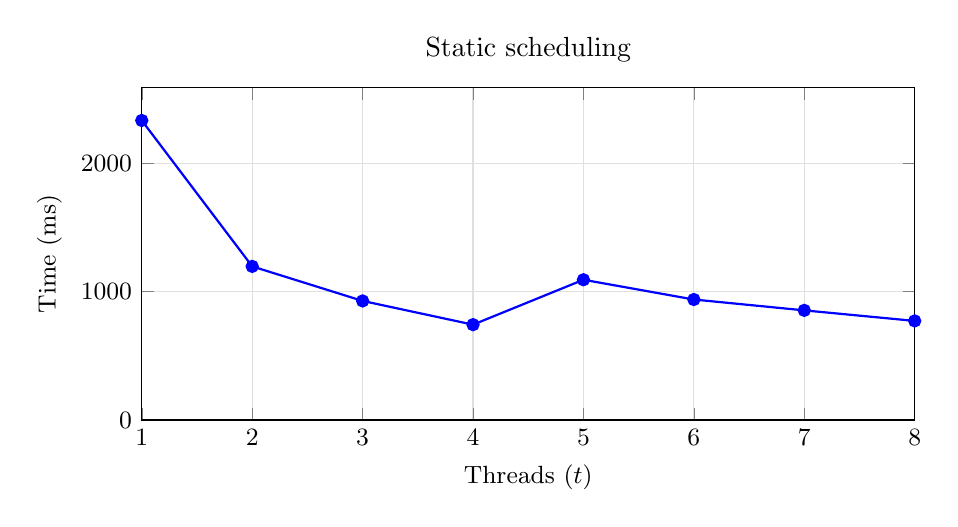
\begin{tikzpicture}
\begin{axis}[width=0.94\linewidth,height=5.8cm,
title={Static scheduling},xlabel={Threads ($t$)},ylabel={Time (ms)},
xmin=1,xmax=8,ymin=0,ymax=2585.23267464,xtick={1,2,3,4,5,6,7,8},
grid=major,major grid style={gray!25},scaled y ticks=false,
tick label style={font=\small},label style={font=\small},
/pgf/number format/1000 sep={}]
\addplot[blue,thick,mark=*,mark size=2pt] coordinates {
(1, 2331.569239)
(2, 1195.889727)
(3, 927.038424)
(4, 742.311509)
(5, 1091.908749)
(6, 938.0144)
(7, 853.580674)
(8, 771.527754)
};
\end{axis}
\end{tikzpicture}
\end{center}
\begin{center}
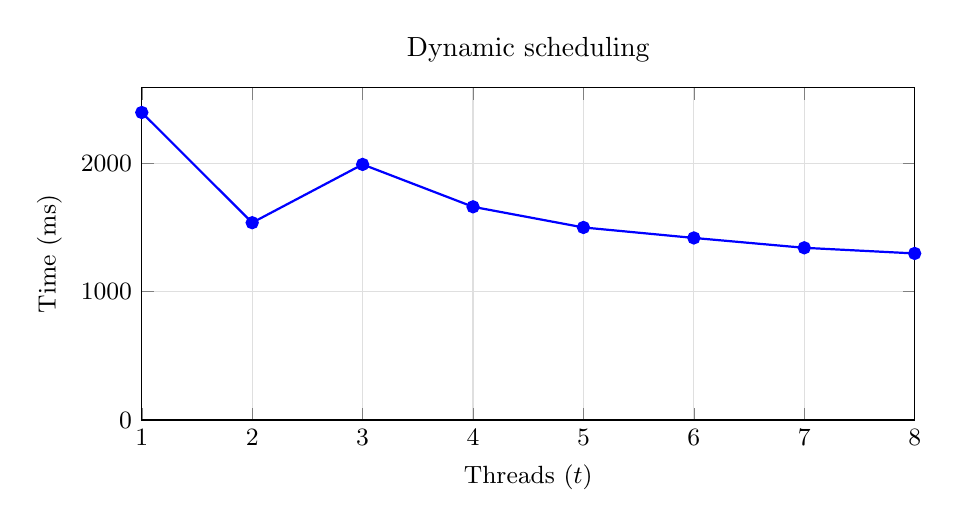
\begin{tikzpicture}
\begin{axis}[width=0.94\linewidth,height=5.8cm,
title={Dynamic scheduling},xlabel={Threads ($t$)},ylabel={Time (ms)},
xmin=1,xmax=8,ymin=0,ymax=2585.23267464,xtick={1,2,3,4,5,6,7,8},
grid=major,major grid style={gray!25},scaled y ticks=false,
tick label style={font=\small},label style={font=\small},
/pgf/number format/1000 sep={}]
\addplot[blue,thick,mark=*,mark size=2pt] coordinates {
(1, 2393.733958)
(2, 1535.909613)
(3, 1989.561264)
(4, 1659.57706)
(5, 1498.833492)
(6, 1417.277686)
(7, 1340.544556)
(8, 1296.621878)
};
\end{axis}
\end{tikzpicture}
\end{center}
\begin{center}
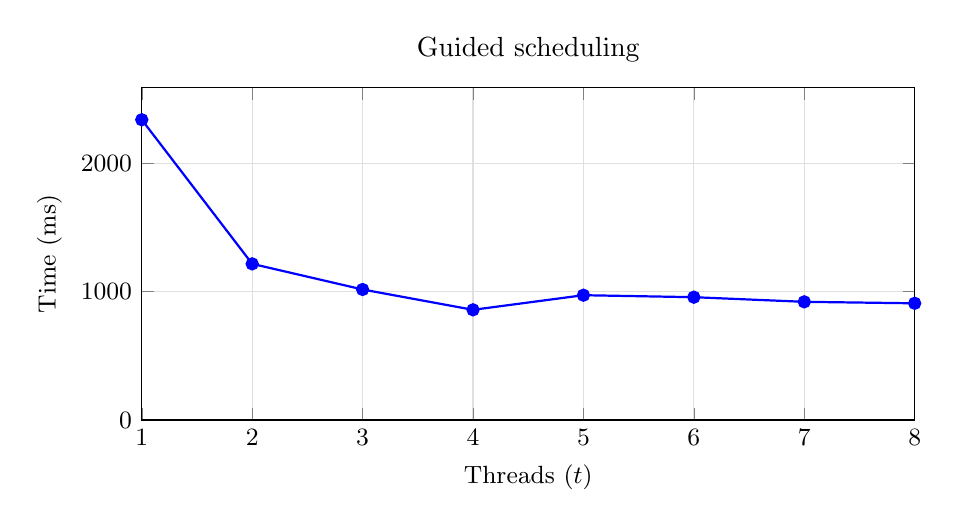
\begin{tikzpicture}
\begin{axis}[width=0.94\linewidth,height=5.8cm,
title={Guided scheduling},xlabel={Threads ($t$)},ylabel={Time (ms)},
xmin=1,xmax=8,ymin=0,ymax=2585.23267464,xtick={1,2,3,4,5,6,7,8},
grid=major,major grid style={gray!25},scaled y ticks=false,
tick label style={font=\small},label style={font=\small},
/pgf/number format/1000 sep={}]
\addplot[blue,thick,mark=*,mark size=2pt] coordinates {
(1, 2337.318849)
(2, 1215.536533)
(3, 1016.097363)
(4, 857.847123)
(5, 971.613289)
(6, 956.106722)
(7, 920.07939)
(8, 908.582073)
};
\end{axis}
\end{tikzpicture}
\end{center}
\end{document}
